\chapter{Future Work}\label{chapter:future_work}

This section presents the future work that can be done to improve the framework proposed while raising energy aware among developers.

The framework presented showed different modules that when combined result in a static analysis tool that estimates energy consumption of Java programs. Each of the modules can have individual improvements that can boost the overall performance of the final extension tool.


\section{Program Generator} \label{sec:future_work_program_generator}

Some improvements can be performed to the Program Generator. The first one is the max input finder. As it is now, the maximum input finder is a simple approach, as it was already explained in Section~\ref{sec:work_stage1_input_tester}. This approach makes it, so it does not find the best combination of inputs available for each method, which can lead to the collected data to avoid edge cases. It is possible to implement a more robust solution that avoids increasing the time complexity by too much, and improves the searching capabilities of the input finder.


%Mambo geral

The final approach uses individually trained models for each method, with each model tailored to its own features and prediction style. But when the dataset grows large enough, there is an opportunity to train a single, more powerful model that can directly estimate methods energy consumption, without needing to run the entire framework every time.
By bringing together the features, predictions, and real energy usage data from all the existing models, this unified model gains access to a richer dataset. That added depth allows it to make accurate energy predictions on its own. Each time the framework processes a method, the resulting model is not just pushed to the extension tool, it also helps improve the centralized model, by making it smarter and more accurate with every update.
While the framework will still handle program generation, energy measurement, and model training for the tool, over time we can consolidate these models towards one powerful model, eliminating the need to run the full pipeline for every new prediction, requiring only parsing the data of the target program and combining with the existing data.


%Building on the progress made so far, additional energy profiles must be created to develop a robust energy inference function. This task involves collecting profiles from different machines and gathering enough data to effectively train the machine learning model. The static analysis tool will be implemented and used to provide important code, specifically, certain features that will feed into the model.

%After that the efforts will be on developing the actual energy inference function. This task is expected to be the most time-consuming, as it is crucial to the tool functioning. It is most likely that this task overlaps the energy profiling task as more profiles might need to be collected. The task will start by implementing the ML algorithms described in \ref{sec:background_machine_learning}, test their accuracy and improving it by tuning the energy profiles for many possible cases.

%When the function is completed, it will be tested against other tools to ensure its quality. The extension will then be built and tested in IDEs.
%While developing the function and the extension, the writing of the thesis will also be done in parallel documenting every information.

%\begin{figure*}%[h]
%  \centering
%  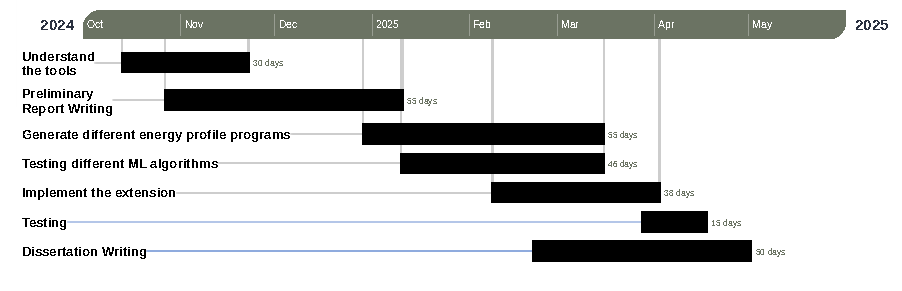
\includegraphics[width = 1 \textwidth]{figures/gantt_diagram.pdf}
%  \caption{Work Plan}
%  \label{fig:gantt_diagram}
%\end{figure*}


%The work plan is illustrated more clearly in Figure \ref{fig:gantt_diagram}, which provides a visual representation of the described tasks. While the dates shown in the figure may not precisely align with the actual timeline, the sequence of tasks remains accurate.